\subsection{Examples of Siumatgwoons}

What are some examples of Siumatgwoons? 



\subsubsection{The Chinese Characters, 字}

The Chinese characters, which inspired this whole mathematical exercise, is clearly a Siumatgwoon. If we exercise the synonym exchange of "Siumatgwoon" with "Metaphysic", then to say the Chinese characters are a siumatgwoon, then this is to say that the Chinese characters is a Metaphysic. 

Unfortunately we can't really \textit{prove} that the Chinese characters are indeed a siumatgwoon, given there's an infinite number of them, and we do not have a generating rule for all Chinese characters. 

However, if given any random subset of all Chinese characters, we can prove that it is a siumatgwoon. 

Let's consider one example. Let's consider the subset of Chinese characters that are composed of only 1 stroke. Consider the following set of Chinese characters: 

$$S=\{\text{日},\text{月}  ,\text{皿},\text{明},\text{盟},\text{盥}\}$$

Let us first verify that this is indeed a siumatgwoon. But here's now an interesting question, how are $*$ and $|$ defined? Well, intuitively, we can say a Chinese character $c = a *b$ if $c$ is made of $a$ and $b$. And we can say that $c|a$ if $c$ appears in the character $a$. Not terribly helpful or illuminating, perhaps - but is this any less illuminating than defining the valuation of $\phi \wedge \psi$ to be the "$0$ unless both the valuation of $\phi$ and the valuation of $\psi$ are $1$"? Tautology is where judgement, human intuition, and the exercise of the human choice to grant admission works, and must work - for logic and mathematics to start. 

One might note there's something seemingly inherently linked to the behaviour of substrings here. If the logic of a siumatgwoon is merely a logic for substrings, which would be plausible since the project of the siumatgwoon appears to be fundemntally a merelogical project, then we might have been rather inflating the intellectual importance of the siumatgwoon. I shall sincerely pray this to not be the case; and I also don't believe this is the case.

So does $S$ satisfy the axioms of a siumatgwoon? 

Axiom \ref{ax:reflexive} says any $s\in S$ satisfies $s|s$. This is clearly true. 
Axiom \ref{ax:total} is clearly true as well. Since there is no character which is simultaneously constituted by two different sets of characters in $S$.

Axiom \ref{ax:transitive} says that for any $s_1, s_2, s_3 \in S$, if $s_1|s_2$ and $s_2|s_3$ then $s_1|s_3$. This is vacuously true, because ha! There are no such three characters in $S$! 

Axiom \ref{ax:composition} says that for any $s_1, s_2 \in S$, $s_1*s_2 \in S$. This is also clearly true - by definition of $*$ and $|$.

So in this very boring example where all 4 axioms are trivially or vacuously true, let us now ask about its atomic set $A$, its elemental set $E$.

Now clearly, we have 
$$A=E=\{\text{日},\text{月},\text{皿}\}$$

So indeed $A\subseteq E$. And indeed in this case, $A=E$, because there are no emergent elements. There are no 系 sets with more than one object - all emergent sets are singletons. This is immediately visible by the fact there are no phonosemanophores 形聲字. And indeed, as proven before, the smallest generator set is indeed $E$, as every object of $S$ is composed by $E$.

And the set of compounds $\{\text{明},\text{盟},\text{盥}\}$ is clearly disjoint from the set of elementals $\{\text{日},\text{月},\text{皿}\}$. 

It is also immediately obvious, that $S$ is a simple siumatgwoon, because no character in $S$ is composed of or constituted by infinitely many other characters in $E$. And clearly, each character is uniquely composed by the elementals, as we can see from the compounds: $\text{盟} =\text{明}*\text{皿} = \text{日}*\text{月}*\text{皿}$.


At this point, it might be really tempting to say if a siumatgwoon is finite, it must be a simple siumatgwoon. But alas, no. We will see this later.


Consider the following siumatgwoon: 
$$S=\{\text{骨}, \text{身}, \text{人}, \text{本}, \text{體}, \text{骵}, \text{躰}, \text{体}\}$$

Let us skip the verification of the axioms, and get to the interesting stuff.

Here, we have 
$$A=\{\text{骨}, \text{身}, \text{人}, \text{本}\}$$
and 
$$E=\{\text{骨}, \text{身}, \text{人}, \text{本}\, text{體}\}$$.


So here, $A\neq E$, because there are emergent elements - phonosemanophores 形聲字. 

What we should immediately point out here is that to the seasoned sinoglyph scholar, he will immediately recognize that 體, 骵,躰,体 are all variants of the same "character", the same "glyph", the same "sign". They point to the same thing. They are \ruby{異體字}{いたいじ}. It is therefore very tempting to then write that the "true form" of $S$ is actually this:



$$S=\{\text{骨}, \text{身}, \text{人}, \text{本}, \text{體} = \text{骵} = \text{躰} = \text{体}\}$$.

Now, if this makes any sense, then we can immediately see that this is not a simple siumatgwoon, because there is a compound with two different decompositions: 


\begin{align}
    \text{體} &= \text{骵} = \text{骨} * \text{身} \\
             &= \text{躰} = \text{身} * \text{本} \\
             &= \text{体} = \text{人} * \text{本}
\end{align}
    
It is still a siumatgwoon. But it is not a simple siumatgwoon. 

One should note that there is something very degenerate in imposing the equality $\text{體} = \text{骵} = \text{躰} = \text{体}$. 

On intuitive and philosophical level, it is not appropriate to write that $\text{體} = \text{骵} = \text{躰} = \text{体}$. The most naive argument is probably that the 4 different glyphs are not really saying the same thing. We are not here to do psychology, but one should consider the psychological and performative motivation behind when one writes $\text{骵}$ instead of $\text{體}$. One is making the point that the referent of $\text{體}$ can actually be decomposed into $\text{骨}$ and $\text{本}$ - that while one party believes $\text{體}$ is an emergent object, the other party believes that $\text{體}$ is actually completely composed by $\text{骨}$ and $\text{本}$ ("a body 體 or 骵 is the basis 本 of a bone 骨" - or some other imaginative formulae involving the 骨 and 本). So in this argument, the two assertions carry different ontological commitments on the nature of what a body is. So $\text{體} \neq \text{骵}$.

This is an interesting argument, but the argument allowing for $\text{體} \neq \text{骵}$ is really intuitively compelling. Obviously, when the champion of the variant writes $\text{骵}$ instead of $\text{體}$ wherever $\text{體}$ appears, say in $\text{身骵}$,$\text{個骵}$,$\text{本骵}$,$\text{人骵}$,$\text{國骵}$,$\text{聖骵}$,$\text{靈骵}$,$\text{天骵}$,$\text{物骵}$, he is clearly making the point that the referent of $\text{體}$ is actually composed by $\text{骨}$ and $\text{本}$. In other words, the referent of $\text{體}$ is the same as the referent of $\text{骵}$. So $\text{體} = \text{骵}$. 

There's also an aesthetic reason why we would be tempted by allowing for $\text{體} = \text{骵} = \text{躰} = \text{体}$, as it seems to allow us this kind of derivation: 

$$\text{骨}, \text{本} \mid \text{骵}$$
$$\text{身}, \text{本} \mid \text{躰}$$
$$\text{人}, \text{本} \mid \text{体}$$
$$\text{骵} = \text{體} = \text{躰} = \text{体}$$
$$\therefore \text{骨}, \text{人}, \text{本}, \text{身} \mid \text{骵}, \text{躰}, \text{体}, \text{體}$$

Well the conclusion that "bone", "man", "base", "body", are all constituents of "body" is very intuitively compelling. It's not yet certain what the rules of reference are employed here, but whatever they are, if this derivation is admitted, then we can then work to formalize those rules of reference, and the logical structure of the mathematical object of Siumatgwoon would be richer for it. 

But this introduces some very degenerate behaviiour into the Siumatgwoon object. The genie responsible is the $=$ relationship. It breaks our semantic definition of $*$ and $|$, as $*$ and $|$ are no longer matters of considering what the substrings of a Chinese character is, because a character like $\text{體}$ can now have "hidden" constituents $ \text{人}, \text{本}, \text{身}$. 

Also, to allow for $=$ in a siumatgwoon, it might introduce certain undesirable set theoretic behaviour. Not quite sure how to demonstrate this, but the potential for violation is intuitively plausible. Notationally, if we allow for $=$, in set theoretic language, the objects $\text{體}, \text{骵}, \text{躰}, \text{体}$ are all just the same object. So notationally, 

$$S=\{\text{骨}, \text{身}, \text{人}, \text{本}, \text{體} = \text{骵} = \text{躰} = \text{体}\}$$.

is the same as 
$$S=\{\text{骨}, \text{身}, \text{人}, \text{本}, \text{體}\}$$.

But that's most definitely not what we want to say. And saying that seriously simplifies the structure that one is trying to describe, however naively.

What one is trying to say, is that there is an object $S$ such that 

$$S=\{\text{骨}, \text{身}, \text{人}, \text{本}, \text{體} , \text{骵}, \text{躰}, \text{体}\}$$.

but the objects $\text{體} , \text{骵}, \text{躰}, \text{体}$ are "identical", "equivalent", in some sense, up to some kind of relation - are variants of the same thing. Given the use of "identical", "equivalent", and the very symbol $=$, it seems very compelling that these objects are related by an equivalence relation - reflexivity, symmetry, and transitivity being the core properties governing them. We shall call their relation "synonymy", represented by the symbol $\sim$. So we can write this instead: 

$$S=\{\text{骨}, \text{身}, \text{人}, \text{本}, \text{體} ~ \text{骵} ~\text{躰} ~\text{体}\}$$.

And so the set theoretic collapse vis-a-vis $=$is avoided. 

The synonymy relation $~$ will open up significant structures of interest for us to explore, which we will do later.

Now, we must ask the question, are there other siumatgwoons aside from the Chinese characters? Why yes, of course. 



\subsubsection{The Roman Numerals $\mathfrak{R}$}

One can clearly see that Roman Numerals $\mathfrak{R}$ are a Siumatgwoon, in the same way that anyone can see that the Chinese characters are a Siumatgwoon. However, to appreciate the characteristics that make it a Siumatgwoon, let us consider the subset of Roman Numerals from 1 to 10, which we shall show to also be a Siumatgwoon.

$\mathfrak{R}_{1,10} = \{I, II, III, IV, V, VI, VII, VIII, IX, X\}$

We will say that for two elements $a,b \in \mathfrak{R}_{1,10}$, $a|b$ iff the glyph $a$ appears in $b$. As such, we can say $I | II$ and $I|III$ as an example, and that $V|IV$ and $X|IX$. 

For any elements $a,b\in \mathfrak{R}_{1,10}$, if the glyphs $ab$ so written together forms a glyph that also appears in $\mathfrak{R}_{1,10}$, then we'd say that $a*b\in \mathfrak{R}$.

Now, it's clear that Ax 1 is satisfied trivially. 

Ax 2 is also satisfied trivially.

Ax 3 is also satisfied. 

Ax 4 is also satisfied. As an example: $I | III, III | VIII$ and we have $I|VIII$.

So therefore, $\mathfrak{R}_{1,10}$ is a Siumatgwoon. 

It is also interesting to note that as per the definition of $\mathfrak{R}_{1,10}$, it is not compositionally closed. For example, $II * III$ is not in $\mathfrak{R}_{1,10}$. This makes the Siumatgwoon different from a group, where all compositions are contained inside the group. Intuitively, perhaps this suggests the Siumatgwoon is less rich in structure than the mathematical group? Also, note that what $II * III$ should be in $\mathfrak{R}_{1,10}$ is represented by $V$. Intuitively, we can feel that in some sense, $II * III = V$ - that they're synonymous, identical, referring to the same referent. This is not unlike the presence of variant characters in the Sinoglyphs, such as 體 (body, object)=骵=躰=体, or信 (trust) = 𬢭 = 伩 = 訫 = 㐰… Intuition should hint that this will yield some interesting structures if we pursue the investigation down this path.

This might feel very unsatisfying, because this is no proof. It is merely an observation. One might therefore be tempted to argue, why can't we find a rule or an algorithm or just a function, that maps all the natural numbers to their Roman Numeral representation? Can we then from that algorithm or function, prove that the Roman Numerals are a Siumatgwoon?


Well let's give it a try. The Roman numeral system is governed by a simple, deterministic algorithm — a greedy function that maps any natural number $n$ to its canonical Roman representation $\mathfrak{r}(n)$. The function operates by iteratively subtracting the largest possible value from $n$ from a fixed, descending list of numeral-value pairs, and appending the corresponding symbol to the output string. For instance, to generate $\mathfrak{r}(1987)$, the algorithm subtracts $1000$ (M), then $900$ (CM), then $50$ (L), followed by three $10$s (XXX), $5$ (V), and finally two $1$s (II), yielding the string **MCMLXXXVII**.

We can define this formally as a function:

$$
\mathfrak{r}(n) = s_{i_1} * s_{i_2} * \cdots * s_{i_k}
$$

such that

$$
n = v_{i_1} + v_{i_2} + \cdots + v_{i_k}, \quad \text{with each } v_{i_j} \in \{1000, 900, 500, \ldots, 1\}
$$

and where $s_{i_j}$ is the Roman numeral glyph corresponding to $v_{i_j}$, chosen at each step to be the largest available $v \leq n$. This ensures that the representation is unique and canonical — a deterministic output of this greedy process.

The same procedure can be extended naturally to represent numbers beyond 3999. Since traditional Roman numerals lack compact notation for such magnitudes, we employ a conventional extension: an overbar denotes multiplication by 1,000. Thus, $\overline{V}$ represents 5000, $\overline{X}$ denotes 10,000, and so forth. In implementation, one may write these as, e.g., `|V|` for clarity in ASCII environments. The algorithm remains unchanged: it continues selecting the largest applicable numeral-value pair (now extended with overbarred forms), subtracting, and appending symbols, until the number is fully decomposed.

Under this construction, not only is there a well-defined function $\mathfrak{r} : \mathbb{N}_{>0} \rightarrow \mathfrak{R}$, but we can also use it to define a **canonical composition operator**:

$$
a * b := \mathfrak{r}(\mathrm{val}(a) + \mathrm{val}(b))
$$

and 

$$a \mid b \iff \text{multiset}(\mathfrak{r}^{-1}(a)) \subseteq \text{multiset}(\mathfrak{r}^{-1}(b))$$
where $\mathrm{val}(a)$ denotes the numeric value of the Roman numeral $a$. That is, composition is interpreted as value-addition followed by re-normalization via the greedy function $\mathfrak{r}$. Constitution $a | b$, in turn, can be rigorously defined as multiset inclusion: $a | b$ iff every glyph used in the canonical decomposition of $a$ appears (with equal or greater multiplicity) in that of $b$.

From here, we can prove — rigorously — that the set of all Roman numerals generated via $\mathfrak{r}$, together with the composition $*$ and constitution $|$, forms a Siumatgwoon. Each of the four axioms holds:

* Reflexivity is immediate: every Roman numeral constitutes itself.
* Totality is trivially satisfied since for any pair $a, b$, either $a$’s multiset of atoms appears in $b$’s or it does not.
* Transitivity follows from transitivity of multiset inclusion.
* Composition Constitution holds because if $c = a * b$, then by construction $c$ is formed from the atoms of both $a$ and $b$, and hence both are constituents of $c$.




Ok, that is very impressive. But the problem is that the algorithm doesn't matter. If the algorithm had been modified such that 57 was not written as LVII but instead as LIIIIIIII, or XXXXXVII or even XXXXX7 or just 57 or @, the resultant object would still be a Siumatgwoon. Even if each of the numbers were represented by their own unique glyph, the resultant object would still be a Siumatgwoon. The underlying generation rule doesn't matter!




\subsubsection{Any Numerals System}

The fact that the Roman Numerals are a Siumatgwoon should intuitively suggest that any numeral system is a Siumatgwoon. In fact, let us consider the world's many numeral systems, and see if there is one where it is not a siumatgwoon. 

\begin{center}
\begin{tabular}{|l|c|c|c|c|c|c|c|c|c|c|}
\hline
 & 0 & 1 & 2 & 3 & 4 & 5 & 6 & 7 & 8 & 9 \\
\hline
唐字數字 & 〇 & 一 & 二 & 三 & 四 & 五 & 六 & 七 & 八 & 九 \\
\hline
唐字數字大寫 & 零 & 壹、弌 & 貳 & 叄 & 肆 & 伍 & 陸 & 柒 & 捌 & 玖 \\
\hline
字喃 &  & 𠬠 & 𠄩 & 𠀧 & 𦊚 & 𠄼 & 𦒹 & 𦉱 & 𠔭 & 𠃩 \\
\hline
蘇州碼子 & 〇 & 〡、一 & 〢、二 & 〣、三 & 〤 & 〥 & 〦 & 〧 & 〨 & 〩 \\
\hline
Roman Numerals &  & I & II & III & IV & V & VI & VII & VIII & IX \\
\hline
Eastern Arabic & ٠ & ١ & ٢ & ٣ & ٤ & ٥ & ٦ & ٧ & ٨ & ٩ \\
\hline
Persian & ٠ & ۰ & ۱ & ۲ & ۳ & ۴ & ۵ & ۶ & ۷ & ۸ \\
\hline
Devanagari & ० & १ & २ & ३ & ४ & ५ & ६ & ७ & ८ & ९ \\
\hline
Gujarati & ૦ & ૧ & ૨ & ૩ & ૪ & ૫ & ૬ & ૭ & ૮ & ૯ \\
\hline
Tibetan & ༠ & ༡ & ༢ & ༣ & ༤ & ༥ & ༦ & ༧ & ༨ & ༩ \\
\hline
Hebrew &  & א & ב & ג & ד & ה & ו & ז & ח & ט \\
\hline
Chinese counting rods &  & 𝍠 & 𝍡 & 𝍢 & 𝍣 & 𝍤 & 𝍥 & 𝍦 & 𝍧 & 𝍨 \\
\hline
counting 正 &  & 𝍲 & 𝍳 & 𝍴 & 𝍵 & 𝍶 & 𝍶𝍲 & 𝍶𝍳 & 𝍶𝍴 & 𝍶𝍵 \\
\hline
Tangut &  & 𘈩 & 𗍫 & 𘕕 & 𗥃 & 𗏁 & 𗤁 & 𗒹 & 𘉋 & 𗢭 \\
\hline
\end{tabular}
\end{center}

I don't think there's a single one that's not a siumatgwoon! Most of them are pathological for sure, in the sense that nothing is constituted by anything else, but none of them violate the Siumatgwoon axioms! 

The case of the numerals as a Siumatgwoon, or a Metaphysic, is interesting. Numerals all refer to the same referents, the same "things" or "objects", namely, numbers. However, the glyphs in a given numeral system are themselves imbued with a particular set of metaphysical prejudices and judgements. Under the Roman Numeral Metaphysic, the number 3 is composed of 1 and 2, or composed of three 1s. 4 is composed of 1 and 5, but not 3 and 2. 

\subsubsection{The Polygons $\mathcal{P}$}

Consider the following graph. If we take all the polygons, convex and star, as elements in a set called $\mathcal{P}$, we can see that it forms a Siumatgwoon. We state this without formal proof for the infinite set $\mathcal{P}$, but from the subset displayed in the graph below, we can see it is indeed true. A polygon $a$ constitutes polygon $b$ if $a$ appears in $b$. $\{3\}$, the equilateral triangle, appears in $\{6/2\}$, the star of David, and so $\{3\} |\{6/2\}$



% include images of polygons_1.png and polygons_2.png
\begin{figure}[!htbp]
    \centering
    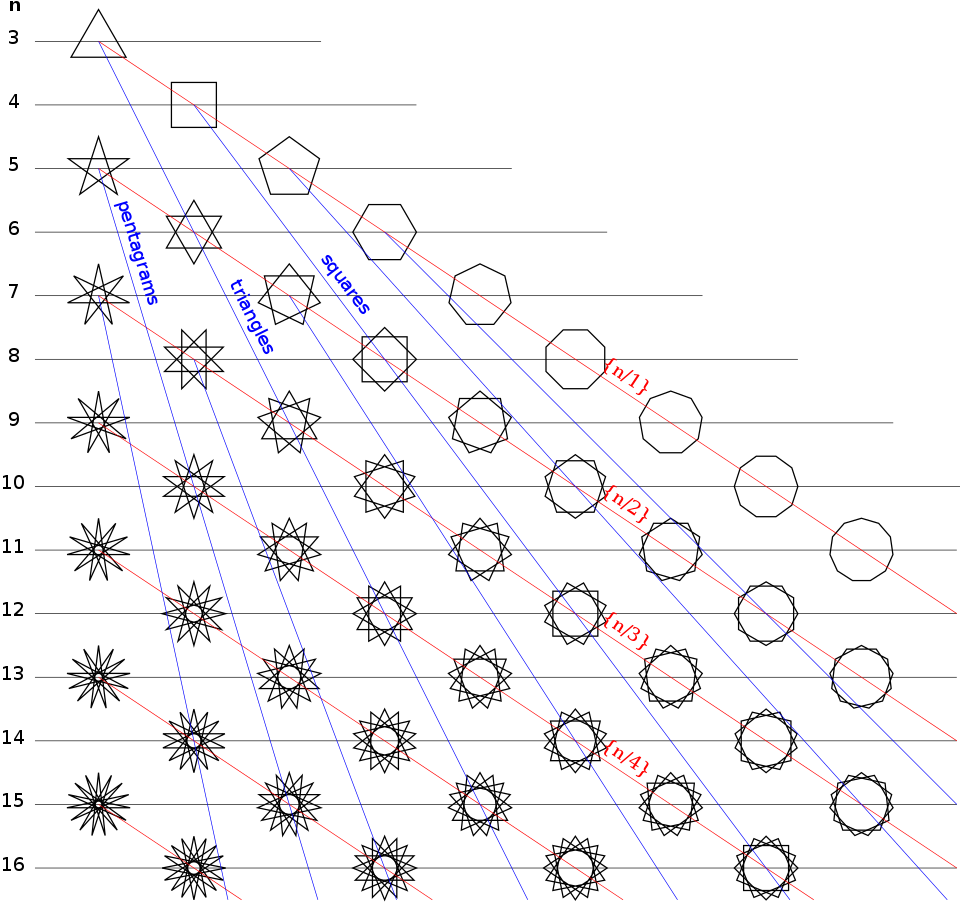
\includegraphics[width=0.8\textwidth]{images/polygons_1.png}
    \caption{A graph of the polygons}
\end{figure}
\begin{figure}[!htbp]
    \centering
    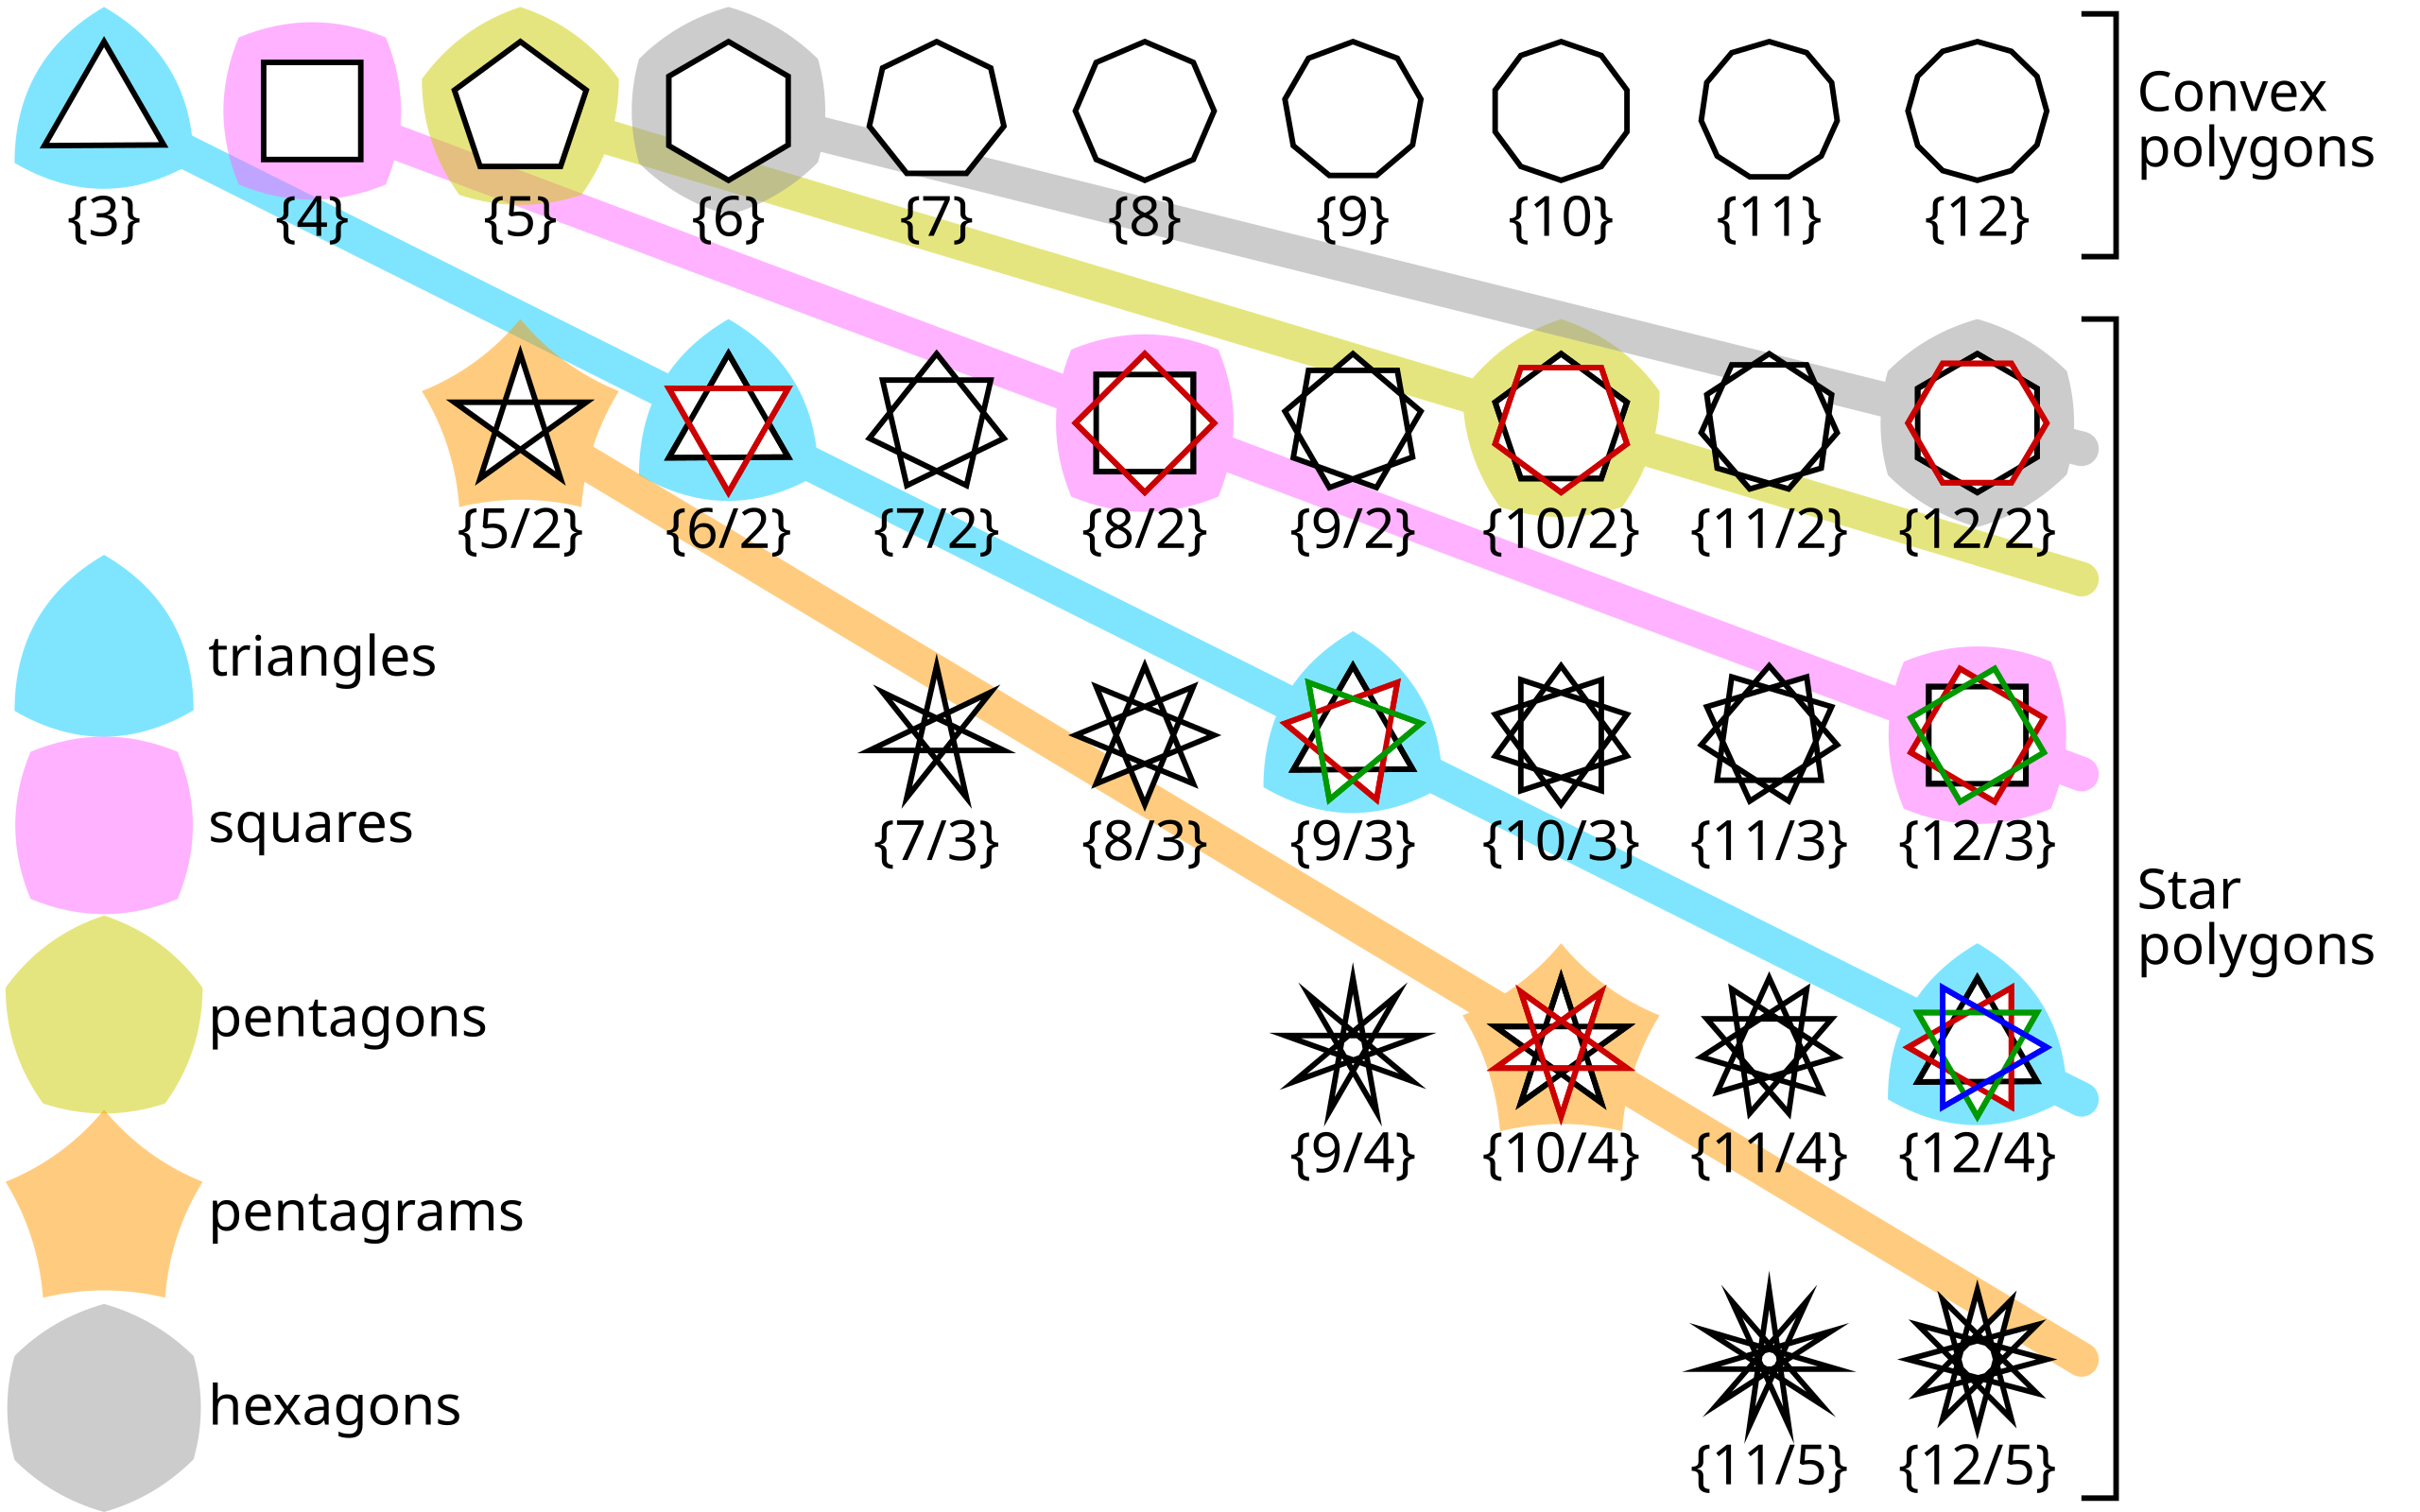
\includegraphics[width=0.8\textwidth]{images/polygons_2.png}
    \caption{A graph of the polygons}
\end{figure}


The Schläfli symbol is a recursive description, starting with $\{p\}$ for a $p$-sided regular polygon that is convex. For example, $\{3\}$ is an equilateral triangle, $\{4\}$ is a square, $\{5\}$ a convex regular pentagon, etc.

Regular star polygons are not convex, and their Schläfli symbols take the form $\{p/q\}$, where $p$ is the number of vertices and $q$ is their turning number. Equivalently, $\{p/q\}$ is created from the vertices of $\{p\}$ by connecting every $q$th vertex. For example, $\{5/2\}$ is a pentagram, while $\{5\}$ is a pentagon.

Note that $p$ and $q$ must be coprime, or the figure will degenerate, in which case we have the following theorem:

$\{p/q\}=d\{ \frac{p}{d} / \frac{q}{d} \}$, where $d=\gcd(p,q)$.

Let us define for any Schläfli symbol $\{p\} | n\{p\}$ for any $n$. It is intuitively true.

Then clearly axiom 1 is satisfied. Axiom 2 is also satisfied.

\subsubsection{Propositional Logic}

There are 3 flavors of $*$ in Propositional Logic: $\wedge, \vee, \rightarrow$. 

And we define $\phi | \psi$ if $\phi$ appears in $\psi$, for any wff $\phi, \psi$.

Then clearly all 4 of the core siumatgwoon axioms are satisfied. 

\begin{enumerate}
\item Trivial that all $\phi | \phi$
\item Also trivial that for any $\phi, \psi$, either $\phi|\psi$ or $\phi\not|\psi$.
\item Trivial as well that for any $\phi,\psi | \phi * \psi$.
\item Also trivial that if $\phi | \psi$ and $\psi | \theta$ then $\phi | \theta$.
\end{enumerate}

Propositional Logic as a Siumatgwoon has multiple interesting properties: 

\begin{enumerate}
\item It is compositionally complete. 
\item It is also constitutionally complete. 
\item Is it a simple siumatgwoon? Are decompositions finite? Yes. Are decompositions unique? Yes, up to reordering. So yes, it's a simple siumatgwoon.


\end{enumerate}

